\documentclass[useAMS,usenatbib]{mn2e}
%\documentclass[twocolumn]{emulateapj}
\usepackage{graphicx,natbib,color,multirow,amsmath}
\voffset=-0.8in

\definecolor{titlecol}{rgb}{0,0,1}
\definecolor{titlecol2}{rgb}{0,0.65,0}
\definecolor{titlecol3}{rgb}{0.99,0.4,0.}

%\definecolor{titledark}{rgb}{0,0,0.8}
%\definecolor{hilit}{rgb}{0,0,1}
%\definecolor{hilitdark}{rgb}{0,0,0.8}
%\font\sbf=cmssbx10 at 32.28pt %big font for headers

\font\nbf=cmssbx10 at 12.28pt %big font for headers

%%%%%%%%%%%%%%%%%%%%%%%%%%%%%%%
%%%% If you want to leave notes in the text feel free to define
%%%% your own colour above and a style below
%%%%%%%%%%%%%%%%%%%%%%%%%%%%%%%
\def\note		{\color{titlecol2} \nbf}
\def\noteb		{\color{titlecol} \nbf}
\def\notebsm	{\color{titlecol}}
\def\notec		{\color{titlecol2} \nbf}
\def\notecsm	{\color{titlecol2}}
\def\notek		{\color{titlecol3} }
\def\builderUC       {} % builder, unconfirmed

%%%%%%%%%%%%%%%%%%%%%%%%%%%%%%%
% For the eventual referee response
\def\changed    {\color{titlecol} }
%\def\changed    {}


%%%%%%%%%%%%%%%%%%%%%%%%%%%%%%%
%  Other stuff I use a lot
\def\oiii		{$\mathrm{\left[ O \textsc{iii}\right] }$}
\def\moiii		{\mathrm{\left[ O \textsc{iii}\right] }}
\def\nii		{$\mathrm{\left[ N \textsc{ii}\right] }$}
\def\mnii		{\mathrm{\left[ N \textsc{ii}\right] }}
\def\sii		{$\mathrm{\left[ S \textsc{ii}\right] }$}
\def\msii		{\mathrm{\left[ S \textsc{ii}\right] }}
\def\galfit     {{\tt GALFIT}}

\def\mmsun	{\rm{M}_{\odot}}
\def\fnobulge    {$f_{\rm no~bulge}$}
\def\mfnobulge {f_{\rm no~bulge}}
\def\fedgeon     {$f_{\rm edge-on}$}
\def\mfedgeon  {f_{\rm edge-on}}
\def\fcnobulge    {$f_{\rm confirmed~no~bulge}$}
\def\mfcnobulge {f_{\rm confirmed~no~bulge}}


%\def\lesssim{\mathrel{\hbox{\rlap{\hbox{\lower5pt\hbox{$\sim$}}}\hbox{$<$}}}}
%\def\gtrsim{\mathrel{\hbox{\rlap{\hbox{\lower5pt\hbox{$\sim$}}}\hbox{$>$}}}}
%new defs of lesssim gtrsim that I think look better
\def\lesssim{\mathrel{\hbox{\rlap{\hbox{\lower3pt\hbox{$\sim$}}}\hbox{\raise2pt\hbox{$<$}}}}}
\def\gtrsim{\mathrel{\hbox{\rlap{\hbox{\lower3pt\hbox{$\sim$}}}\hbox{\raise2pt\hbox{$>$}}}}}


\newcommand\nodata{ ~$\cdots$~ }




\begin{document}

\title[Galaxy Zoo: CANDELS Data Release]{Galaxy Zoo: Detailed Morphological Classifications for 48,000 galaxies from CANDELS\thanks{This publication has been made possible by the participation of more than {\notebsm COUNT} volunteers in the Galaxy Zoo project. Their contributions are
individually acknowledged at http://authors.galaxyzoo.org/ .} } 

\author[Simmons et al.]{\parbox[t]{16cm}{B. D. Simmons$^{1}\thanks{E-mail: brooke.simmons@astro.ox.ac.uk}$, {\notebsm and a \emph{lot} of other people to be named later}
%Chris Lintott$^{1,3}$, 
%Kyle W. Willett$^{5}$, 
%Karen L. Masters$^{2,4}$, 
%Robert C. Nichol$^{2,4}$, 
%William C. Keel$^{6}$, 
%Thomas Melvin$^{2}$, 
%R. J. Smethurst$^{1}$, 
%Edmond Cheung$^{7}$, 
%Kevin Schawinski$^{8}$, 
%Michael Rutkowski$^{5}$,
%Jeyhan S. Kartaltepe$^{9,}$\footnote{Hubble Fellow}, 
%Kevin R. V. Casteels$^{11}$, 
%Christopher J. Conselice$^{12}$,
%Omar Almaini$^{12}$, 
%Henry C. Ferguson$^{13}$,
%Lucy Fortson$^{5}$, 
%William Hartley$^{12,8}$, 
%Dale Kocevski$^{14}$,
%Anton M. Koekemoer$^{13}$,
%Daniel H. McIntosh$^{15}$,
%Alice Mortlock$^{12}$, 
%{\builderUC Jeffrey A. Newman$^{16}$,}
%Jamie Ownsworth$^{12}$, 
%Steven Bamford$^{12}$,
%{\builderUC Tomas Dahlen$^{13}$,} 
%{\builderUC Sandra M. Faber$^{17}$,}
%{\builderUC Steven L. Finkelstein$^{18}$,} 
%{\builderUC Adriano Fontana$^{19}$,}
%{\builderUC Audrey Galametz$^{19}$,}
%N. A. Grogin$^{13}$,
%{\builderUC Ruth Gr\"utzbauch$^{12, 20}$,} 
%{\builderUC Yicheng Guo$^{17}$,}
%{\builderUC Boris H\"au\ss ler$^{12,21,1}$,}
%Kian Jek$^{22}$,
%Sugata Kaviraj$^{21}$,
%Ray A. Lucas$^{13}$,
%{\builderUC Michael Peth$^{23}$,}
%{\builderUC Mara Salvato$^{24}$,} 
%{\builderUC Tommy Wiklind$^{25}$,} 
%{\builderUC Stijn Wuyts$^{24}$}
%
\vspace{0.1in} }\\
$^{1}$Oxford Astrophysics, Denys Wilkinson Building, Keble Road, Oxford OX1 3RH, UK\\
%$^{2}$Institute of Cosmology \& Gravitation, University of Portsmouth, Dennis Sciama Building, Portsmouth PO1 3FX, UK\\
%$^{3}$Adler Planetarium, 1300 S. Lake Shore Drive, Chicago, IL 60605, USA\\
%$^{4}$SEPnet,\thanks{www.sepnet.ac.uk} South East Physics Network\\
%$^{5}$School of Physics and Astronomy, University of Minnesota, 116 Church St. SE, Minneapolis, MN 55455, USA\\
%$^{6}$Department of Physics and Astronomy, University of Alabama, Box 870324, Tuscaloosa, AL 35487, USA\\
%$^{7}$Department of Astronomy and Astrophysics, 1156 High Street, University of California, Santa Cruz, CA 95064, USA\\
%$^{8}$Institute for Astronomy, ETH Z\"urich, Wolfgang-Pauli-Strasse 27, CH-8093 Z\"urich, Switzerland\\
%$^{9}$National Optical Astronomy Observatory, 950 N. Cherry Ave., Tucson, AZ, 85719, USA\\
%$^{10}$Department of Astronomy, University of Michigan, Ann Arbor, MI 48104, USA\\
%$^{11}$Institut de Cincies del Cosmos. Universitat de Barcelona (UB-IEEC), Mart i Franqus 1, E-08028 Barcelona, Spain\\
%$^{12}$School of Physics \& Astronomy, University of Nottingham, Nottingham NG7 2RD\\
%$^{13}$Space Telescope Science Institute, 3700 San Martin Drive, Baltimore, MD 21218\\
%$^{14}$Department of Physics and Astronomy, University of Kentucky, Lexington, KY 40506, USA\\
%$^{15}$Department of Physics, University of Missouri-Kansas City, 5110 Rockhill Road, Kansas City, MO 64110, USA\\
%$^{16}$Department of Physics and Astronomy \& PITT PACC, University of Pittsburgh, Pittsburgh, PA 15217, USA\\
%$^{17}$UC Observatories/Lick Observatory and Department of Astronomy and Astrophysics, University of California, Santa Cruz, CA 95064, USA\\
%$^{18}$Department of Astronomy, The University of Texas at Austin, Austin, TX 78712, USA\\
%$^{19}$INAF-Osservatorio Astronomico di Roma, Via Frascati 33, I-00040, Monteporzio, Italy\\
%$^{20}$Centre for Astronomy and Astrophysics, University of Lisbon, P-1349-018 Lisbon, Portugal\\
%$^{21}$Centre for Astrophysics Research, University of Hertfordshire, College Lane, Hatfield AL10 9AB, UK\\
%$^{22}$Galaxy Zoo Volunteer\\
%$^{23}$Department of Physics and Astronomy, The Johns Hopkins University, Baltimore, MD 21218, USA\\
%$^{24}$Max-Planck-Institut f{\"u}r extraterrestrische Physik, Giessenbachstrasse 1, D�85748 Garching bei M{\"u}nchen, Germany\\
%$^{25}$European Southern Observatory/Joint ALMA Observatory, 3107 Alonso de Cordova, Santiago, Chile\\
   }

\maketitle
  
\label{firstpage}
  
%\clearpage

\begin{abstract}

{\notebsm To be rewritten, probably last.}

Galaxies are sometimes really far away. The distant ones are pretty cool, because they tell us what the Universe was like back when it was just a kid, or maybe a teenager. You really have to look hard to see these galaxies, but once you do, what you do see tells you a whole lot. I mean, it's not exactly a WYSIWYG type of thing: there's a lot of work to figure out what the faint stuff you see really means. We did a bunch of work, and we think we did pretty well. Also, we compared to others who have done different kinds of work to try and answer some of the same questions. But we have a unique way of answering them, so here are those answers, and you can use them to answer other questions about the Universe.


  \end{abstract}
  
  \begin{keywords}
  
  galaxies: general 
  --- 
  galaxies: evolution
  --- 
  galaxies: morphology %not actually a keyword 
  --- 
  galaxies: structure
  
  \end{keywords}

%%%%%%%%%%%%%%%%%%%%%%%%%%%%%%%%%%%%%%%%%%%%%%
%
%  
\section{Introduction}
%
%
%%%%%%%%%%%%%%%%%%%%%%%%%%%%%%%%%%%%%%%%%%%%%%

{\notebsm Outline:}\\
Galaxy morphologies trace physics \& dynamics and are therefore important.

They have a long history and there are many types, including those that use proxies [which are useful but not without problems] and those that reduce a galaxy and its billions of stars to a single number [same]. Visual morphologies are in many ways still ideal as they are able to provide incredibly detailed information about galaxies.

Visual morphologies have a scale problem without many eyes, and they're often not quantified. Galaxy Zoo to the rescue.

Galaxy Zoo started in 2007 and has provided robust, quantified visual classifications for more than 1,000,000 galaxies to $z \sim 1$. 

Much use has been made of these, including [summarize and include non-GZ papers].

Here we present the visual morphologies of galaxies imaged by the $HST$ treasury survey CANDELS.

Section summary and cosmology.




%%%%%%%%%%%%%%%%%%%%%%%%%%%%%%%%%%%%%%%%%%%%%%
%
%
\section{Observational Data}\label{sec:data}
%
%
%%%%%%%%%%%%%%%%%%%%%%%%%%%%%%%%%%%%%%%%%%%%%%

\subsection{Images}\label{sec:images}

% Note this is lifted directly from the bar paper so I should probably mix it up a bit later
The Cosmic Assembly Near-infrared Extragalactic Legacy Survey \citep[CANDELS;][]{grogin11,koekemoer11} is an \emph{HST} Treasury programme combining optical and near-infrared imaging from the Advanced Camera for Surveys (ACS) and Wide Field Camera 3 (infrared channel; WFC3/IR) across five well-studied survey fields {(GOODS-North and -South, \citeauthor{giavalisco04} \citeyear{giavalisco04}; EGS, \citeauthor{davis07} \citeyear{davis07}; UDS, \citeauthor{lawrence07} \citeyear{lawrence07}, \citeauthor{cirasuolo07} \citeyear{cirasuolo07}; and COSMOS, \citeauthor{scoville07} \citeyear{scoville07}) using a two-tiered ``deep'' and ``wide'' approach. Each of the wide fields (UDS, COSMOS, EGS and flanking fields to the GOODS-S and GOODS-N deep fields) are imaged over 2 orbits in WFC3/IR, split in a 2:1 ratio between filters F160W and F125W, respectively, with parallel exposures in F606W and F814W using ACS. Each of the deep fields (GOODS-S and GOODS-N) are imaged over at least 4 orbits each in both the F160W and F125W filters and 3 orbits in the F105W filter, with ACS exposures in F606W and F814W in parallel. These are reduced and combined to produce a single mosaic for each field in each band, with drizzled resolutions of $0.03^{\prime\prime}$ and $0.06^{\prime\prime}$ per pixel for ACS and WFC3/IR, respectively \citep[a process described in detail by][]{koekemoer11}.

Here we use the CANDELS ACS and WFC3/IR images from within the first set of data to be classified within the Galaxy Zoo interface. Those data cover the COSMOS, GOODS-South, and UDS fields. The 4th release of Galaxy Zoo included all detections with $H \leq 25.5$ from these 3 combined fields, comprising 49,555 unique images. These were shown to visitors to the website galaxyzoo.org{\footnote{Archived at zoo4.galaxyzoo.org}} starting on the 10th of September, 2012.  

The images shown to the public are colour composites of ACS $I$ ($F814W$), WFC3 $J$ ($F125W$), and WFC3 $H$ ($F160W$) filters for the blue, green and red channels, respectively. The angular sizes of the images in different filters are matched, and the native point-spread functions (PSFs) are used. The images are combined with an asinh stretch \citep[described in detail in][]{luptonasinh} with a non-linearity value of {\notebsm 3.0}. 

Sources in the dataset vary greatly in size and surface brightness, and therefore a single set of values for channel scalings is not adequate to capture the variety of features across the images. We therefore use a variable scaling based on the {\notebsm magnitude and size} of each target source. For each image the R, G, and B channels have a fixed ratio of {\notebsm [not sure; must get this from Jeyhan]}, and the multiplier can vary between {\notebsm A and B}. Figure \ref{fig:imageexamples} shows examples of these colour composites across a wide range of source fluxes and sizes. 

Each colour image is 424 pixels square. The angular size of the image varies, such that the colour image encompasses at least {\notebsm 3 times the 80\% flux radius of the target source}, with a minimum screen-to-WFC3 zoom ratio of {\notebsm 1:10} and a maximum ratio of {\notebsm 3:1}. The Galaxy Zoo interface loads the normal colour images by default, and the user may choose to display an inverted colour image, but may not otherwise change the image scaling or size within the software while performing the classification.



\subsection{Photometry}


Brief description of photometric catalogs. Focus on $IJH$ because that's all the images consider. Do mention all the extra stuff available, but note that the classifications themselves don't depend on them.
%The debiasing will, though, because the photometric redshifts do.



\subsection{Redshifts}\label{sec:z}

Some of them have speczs. Lots of them have photzs, including CANDELS, 3D-HST and several previous surveys.
%I'm thinking the first thing to do is pick a redshift for all the sources, and settle on it, before any other analysis proceeds.
%Also it would be helpful to match each ID we use to the CANDELS unique ID that the team uses. Even if we don't publish it.

Comparison of photozs and speczs; might be able to just reference the other papers.

What do we do about those without redshifts? We use them with caution?


%%% I'm taking this out because at the moment we aren't using these
%\subsection{Simulated Images}\label{sec:ferengi}

%Describe simulations and what we'll use them for.




%%%%% [FIGURE: Bar fractions and mags of sample] %%%%%
%\begin{figure*}
%\includegraphics[scale=0.273]{tree_part_with_selection.eps}
%\caption{
%\emph{Left:} Partial Galaxy Zoo: CANDELS classification tree, starting with the first question (top) and leading to the bar feature question. There are 17 questions total in the tree; the bar question is a 4th-tier task. \emph{Right:} Selection of the featured, not-edge-on disk galaxy sample (876 galaxies) in GZ-CANDELS; relative box areas are scaled to the sample sizes. This selection was made independently of restrictions on redshift or luminosity (a full description of the sample selection is given in Section \ref{sec:sample}). Eight independent classifiers subsequently examined each of the 876 disk galaxies for evidence of a bar. 
%}
%\label{fig:sampleselection}
%\end{figure*}
%%%%% END FIGURE %%%%%




%%%%% [FIGURE: Example images] %%%%%
%\begin{figure*}
%\includegraphics[scale=1.0]{barfig_3.eps}
%\caption{
%Examples of disk galaxies in GZ-CANDELS whose bar vote percentage $(p_{bar})$ places them in the unbarred (top row) and barred (bottom row) sub-samples.
%}
%\label{fig:gals}
%\end{figure*}
%%%%% END FIGURE %%%%%


\subsection{Calibration and Simulated Images}

Mention the duplicated images in GDS, which were put in both identically (this was by accident - so we got double each of these and can theoretically check the variance in classifications, but that's kind of a stupid justification and I'm not quite sure how to mention these without saying "oopsies") and at 2-epoch depth (though this has not actually happened yet so I may need to just leave it out). Also it'd be nice to mention the FERENGIfied images, but ... those aren't in yet either. Basically, the only reason to have this section at the moment is to say "oops".



%%%%%%%%%%%%%%%%%%%%%%%%%%%%%%%%%%%%%%%%%%%%%%
%
%
\section{Classification Data}\label{sec:classifications}
%
%
%%%%%%%%%%%%%%%%%%%%%%%%%%%%%%%%%%%%%%%%%%%%%%

\subsection{Decision Tree}

%%%%% [FIGURE: Example images] %%%%%
\begin{figure*}
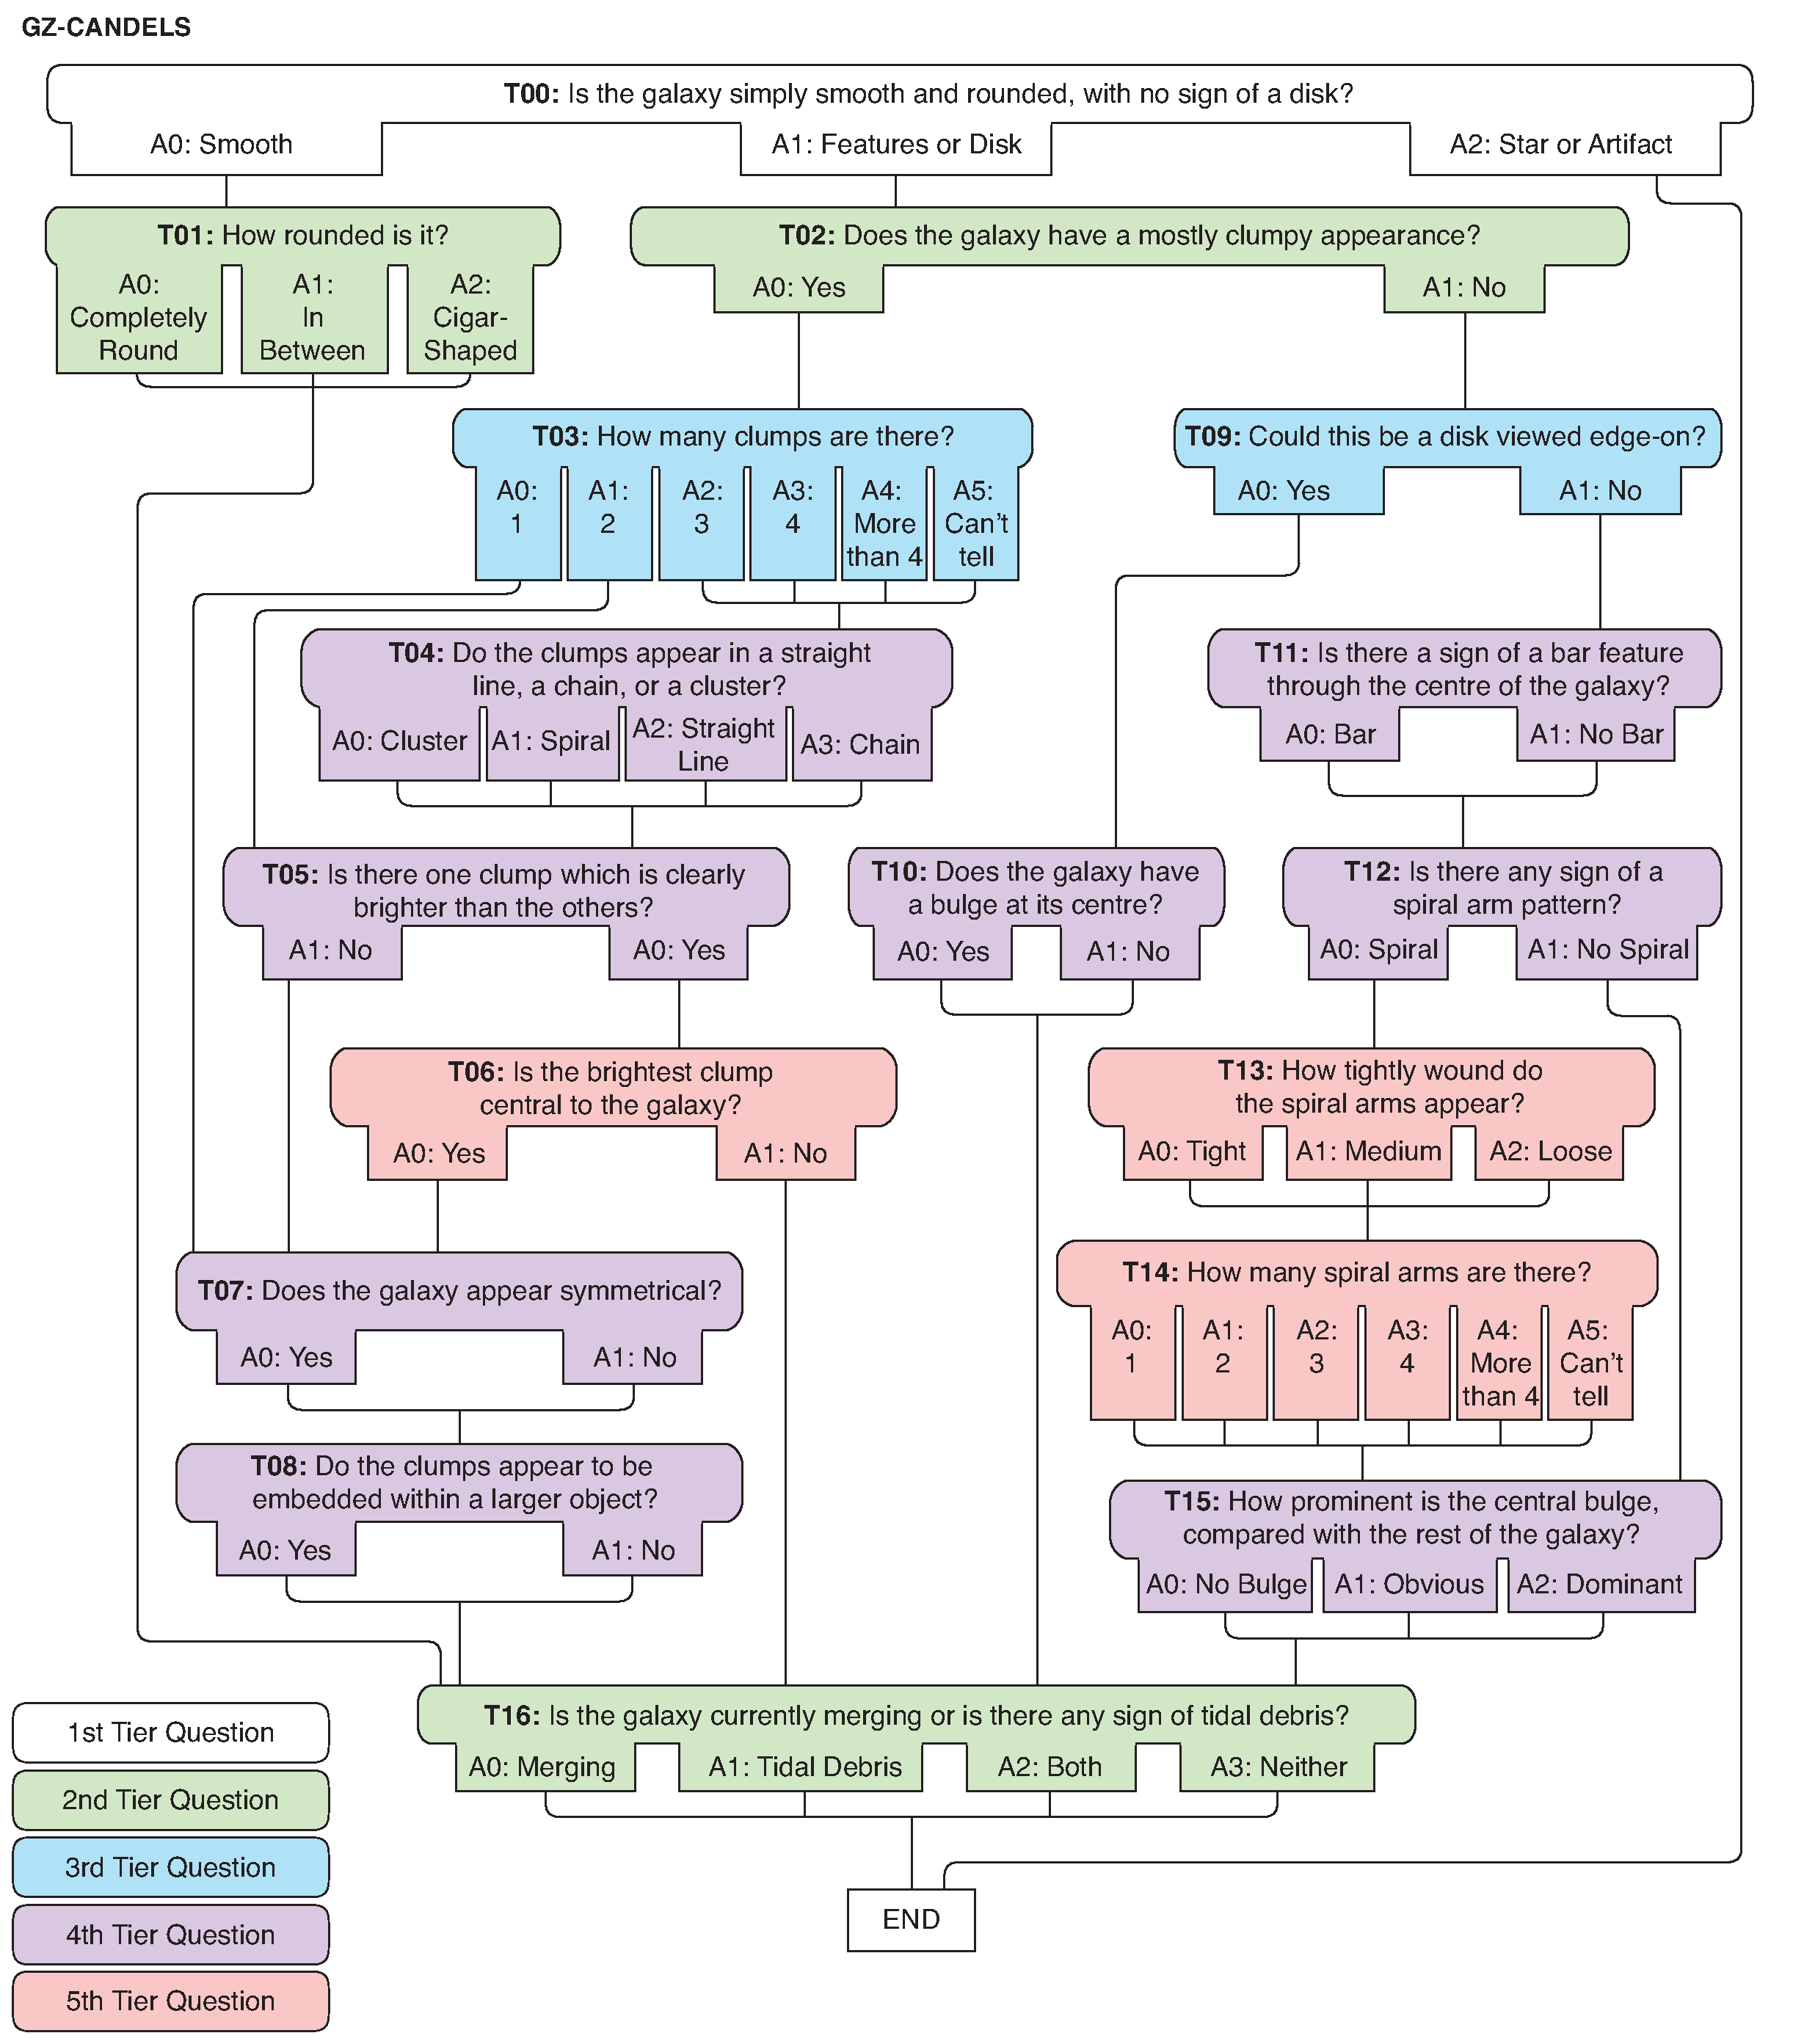
\includegraphics[scale=0.45]{candels_classification_tree_withlabels_new.eps}
\caption{
The Decision Tree for Galaxy Zoo: CANDELS in visual format. There are 16 tasks, with one question per task and up to 6 answers per question. Questions are coloured according to the minimum number of branches prior to that question. All users are asked the first question (task T00), and there are 4 subsequent levels of branching. The tree is also shown in text in Table \ref{table:tree}.
}
\label{fig:tree}
\end{figure*}
%%%%% END FIGURE %%%%%

The goal of Galaxy Zoo CANDELS is to provide detailed quantitative visual morphologies of galaxies observed by the deepest, most complete \emph{HST} multi-wavelength legacy survey to date. 
%The classification interface was designed first and foremost with this goal in mind. 
There are many morphological features of interest, including both broad questions about a galaxy's overall appearance and more detailed questions about specific features. 

We employ a tree-based structure for collecting information on these morphological features, a strategy that has been used successfully in both Galaxy Zoo 2 {\notebsm (refs here)} and Galaxy Zoo: Hubble {\notebsm (and here)}. The decision tree, shown visually in Figure \ref{fig:tree} and in text in Table \ref{table:tree}, first asks the classifier to choose between the broad categories of "smooth and rounded", "features or disk", and "star or artifact". The next question either exits the classification (if the classifier has indicated the image is of a star or artifact) or asks for further details about the galaxy. 

If the classifier has indicated in the first question that the galaxy has features or a disk, a series of follow-up questions are asked about features such as clumps, spiral patterns, bulge strength, and the presence of a bar. If the classifier has instead indicated the galaxy is mostly smooth and rounded, the next question asks them to rate the overall roundedness, a question roughly corresponding to an axis ratio measurement. Finally, when the classifier has finished answering all follow-up questions about either the "smooth" or "featured" galaxy, they are then asked whether the galaxy is undergoing a merger, has tidal tails, or has both, or neither.

The tree-based structure has a number of advantages. First, it collects substantially more information on each galaxy than a single question would, and captures a more detailed classification of higher-order structures while minimising the effort required on the part of the classifier by only asking for relevant inputs based on the answers provided to previous questions. 

Second, it focuses the classifier on a single feature at a time, highlighting each feature. This resets the attention of the classifier with each new question and avoids the problems that may result when a person is presented with a large number of decision tasks at once, including a decrease in optimal decision-making {\notebsm (references for overchoice)} and a reduced ability to recognise the unexpected {\notebsm (references for inattentional blindness)}. 

Third, the tree-based structure is especially optimal for an interface which may collect classifications from users who have never before seen an image of a galaxy and may seek additional training. Within the interface, the classifier may optionally display training images in a ``Help'' section that shows different examples of the feature relevant to the current question. Asking single-topic questions in turn permits a full set of training images to be available throughout the classification without placing an unnecessary cognitive load on the classifier.

{\notebsm Other advantages we should mention?}

The disadvantage of a tree-based classification structure concerns the dependencies introduced into the vote fractions by such a structure. A classifier cannot, for example, answer that the same galaxy has both a mostly smooth appearance and also has a spiral feature. This is in some ways an advantage, as it prevents contradictory and unphysical classifications, but it also means that an analysis of  morphological vote fractions with the goal of examining spiral galaxies must account for the fact that whether a given classifier reached the spiral branch of the decision tree depends on their answer to the questions preceding it. 

Accounting for dependencies of questions in deeper branches of the decision tree on higher-level questions is, however, a manageable task which has been undertaken successfully in many previous studies of specific galaxy structural features {\notebsm {(for specific examples, see [citation bomb here])}}. 

The Galaxy Zoo CANDELS decision tree is shown in visual form in Figure \ref{fig:tree} and in text form in Table \ref{table:tree}. We note that this tree is most similar to the tree used in the Galaxy Zoo: Hubble project \citep[shown in ][]{melvin14} {\notebsm (note to self to check that the full tree is actually shown there)}, which also has an additional branch identifying clumpy galaxies and focusing on the detailed structure of galaxy clumps. There are small differences, however: for example, Task 10, the question about a bulge in an edge-on disk, is a Yes/No question here, whereas in previous iterations of the decision tree this question also asked whether the bulge shape was rounded or boxy. Additionally, the final question in the tree (Task 16) is substantially different from previous versions and is here only concerned with galaxy mergers and tidal features. 

After the classification of each image is finished, the classifier is asked "Would you like to discuss this object?" If the classifier selects "No", a new image is shown for classification. If the classifier selects yes, a new window opens with a discussion page focused on the image they have just classified. Within this part of the Galaxy Zoo software, called Talk, users may ask questions and make comments on specific images, or engage in more general discussions. Users may also "tag" images and discussions using a format identical to Twitter's hashtag system. Some of these tags were used in the pre-analysis of Galaxy Zoo CANDELS data, on which more details are given in Section \ref{sec:dunno} below.



\begin{table}
 \begin{tabular}{@{}cllr}
 \hline
\multicolumn{1}{l}{Task} &
\multicolumn{1}{c}{Question} &
\multicolumn{1}{c}{Responses} &
\multicolumn{1}{c}{Next} 
\\ 
\hline
\hline						
T00    & {\it Is the galaxy simply smooth   }  & smooth           & 01 \\
      & {\it and rounded, with no sign of  }  & features or disk & 02 \\
      & {\it a disk?                       }  & star or artifact & {\bf end} \\
      \hline
T01    & {\it How rounded is it?            }  & completely round & 16 \\
      & {\it                               }  & in between       & 16 \\
      & {\it                               }  & cigar-shaped     & 16 \\
      \hline
T02    & {\it Does the galaxy have a    }  & yes                  & 03 \\
      & {\it mostly clumpy appearance? }  & no                   & 09 \\
      \hline
T03    & {\it How many clumps           }  & 1                    & 07 \\
      & {\it are there?                }  & 2                    & 05 \\
      & {\it                           }  & 3                    & 04 \\
      & {\it                           }  & 4                    & 04 \\
      & {\it                           }  & more than four       & 04 \\
      & {\it                           }  & can't tell           & 04 \\
      \hline
T04    & {\it Do the clumps appear in   }  & cluster              & 05 \\
      & {\it a straight line, a chain  }  & spiral               & 05 \\
      & {\it or a cluster?             }  & straight line        & 05 \\
      & {\it                           }  & chain                & 05 \\
      \hline
T05    & {\it Is there one clump which is       }  & yes          & 06 \\
      & {\it clearly brighter than the others? }  & no           & 07 \\
      \hline
T06    & {\it Is the brightest clump    }  & yes                  & 07 \\
      & {\it central to the galaxy?    }  & no                   & 16 \\
      \hline
T07    & {\it Does the galaxy           }  & yes                  & 08 \\
      & {\it appear symmetrical?       }  & no                   & 08 \\
      \hline
T08    & {\it Do the clumps appear to be       }  & yes           & 16 \\
      & {\it embedded within a larger object? }  & no            & 16 \\
      \hline
T09    & {\it Could this be a disk viewed   }  & yes              & 10 \\
      & {\it edge-on?                      }  & no               & 11 \\
      \hline
T10    & {\it Does the galaxy have a        }  & yes              & 16 \\
      & {\it bulge at its centre?          }  & no               & 16 \\
      \hline
T11    & {\it Is there a sign of a bar      }  & bar              & 12 \\
      & {\it feature through the centre    }  & no bar           & 12 \\
      & {\it of the galaxy?                }                          \\
      \hline
T12    & {\it Is there any sign of a        }  & spiral           & 13 \\
      & {\it spiral arm pattern?           }  & no spiral        & 15 \\
      \hline
T13    & {\it How tightly wound do the      }  & tight            & 14 \\
      & {\it spiral arms appear?           }  & medium           & 14 \\
      & {\it                               }  & loose            & 14 \\
      \hline
T14    & {\it How many spiral arms          }  & 1                & 15 \\
      & {\it are there?                    }  & 2                & 15 \\
      & {\it                               }  & 3                & 15 \\
      & {\it                               }  & 4                & 15 \\
      & {\it                               }  & more than four   & 15 \\
      & {\it                               }  & can't tell       & 15 \\
      \hline
T15    & {\it How prominent is the          }  & no bulge         & 16 \\
      & {\it central bulge, compared       }  & just noticeable  & 16 \\
      & {\it with the rest of the galaxy?  }  & obvious          & 16 \\
      & {\it                               }  & dominant         & 16 \\
      \hline
T16    & {\it Is the galaxy currently       }  & merging          & {\bf end}  \\
      & {\it merging or is there any       }  & tidal debris     & {\bf end}  \\
      & {\it sign of tidal debris?         }  & both             & {\bf end}  \\
      & {\it                               }  & neither          & {\bf end}  \\
      \hline
 \end{tabular}
 \caption{The Galaxy Zoo CANDELS decision tree, comprising 16 tasks and 51 responses. Each task is comprised of a single question and up to 6 possible responses. The first question is Task 00, and a classification is completed by responding to all subsequent questions until the end of the tree is reached. The `Next' column indicates the subsequent task the classifier is directed to upon choosing a specific response. Although a classifier will flow through the tree from top to bottom, there is no path through the tree that includes all tasks. 
%The texts in `Question' and `Responses' are displayed to volunteers during classification, along with the icons in Figure~\ref{fig-flowchart}.
\label{table:tree}}
\end{table}



\subsection{Raw classifications}

% First classification 2012-09-10 18:41:25 UTC, last classification 2013-11-30 12:58:51 UTC
% NOTE I've just discovered that people who put commas in their usernames can mess up my (admittedly simple and awk-based) system of separating classifications. 
% So I am 99% sure the total number of classifications is 2,149,206 but I'm not 100% sure yet.

%%%%% [FIGURE: Example images] %%%%%
\begin{figure*}
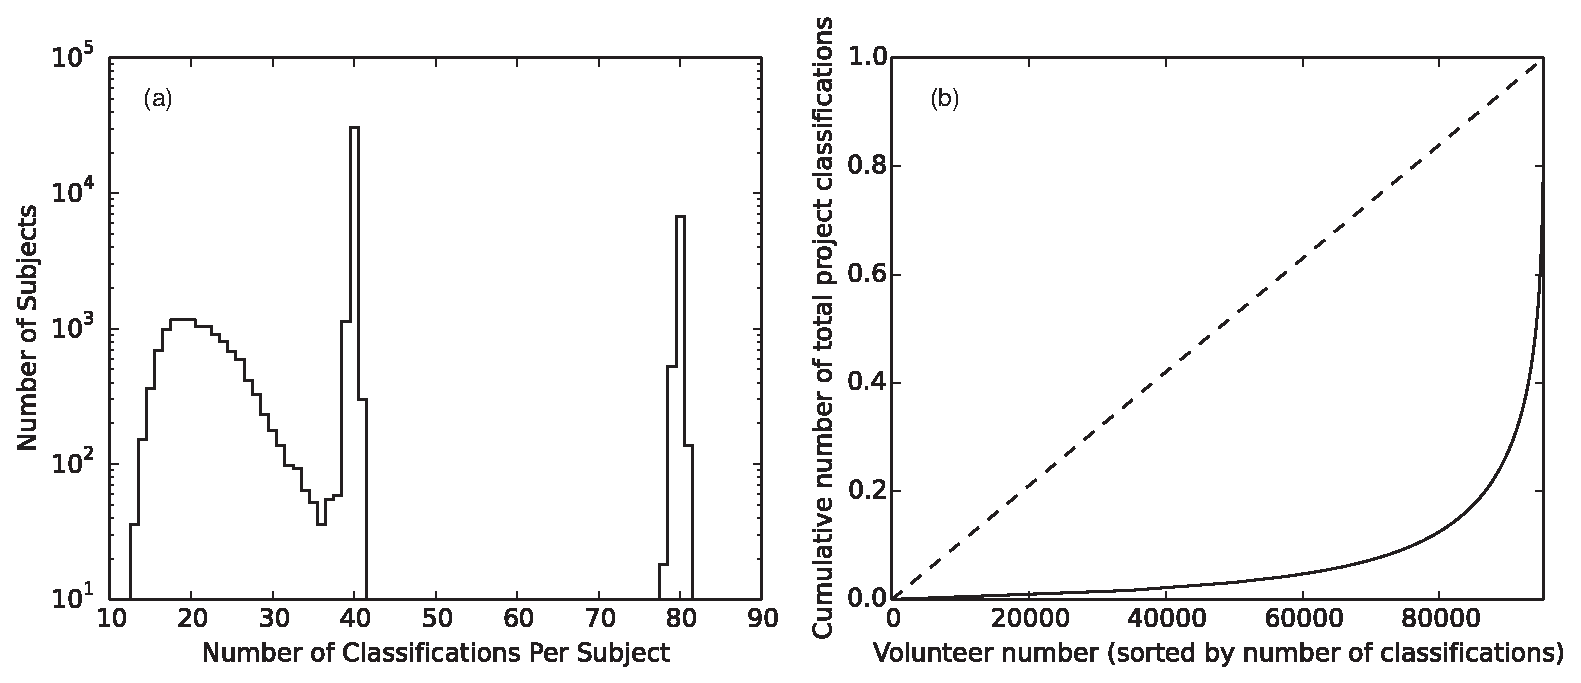
\includegraphics[scale=0.67]{classifications_users_basicinfo.eps}
\caption{
Basic information on classifications. \emph{Left}: Distribution of number of classifications per subject in Galaxy Zoo CANDELS. The majority of images have 40 independent classifications each; a subset of 13,392 were retired early after being identified as too faint and low-surface-brightness for additional classifications to be useful (11,837) or as stars or artifacts (1,555). Subsequently, 7,402 subjects where at least 20\% of classifiers registered a vote for ``Features or Disk'' in the first task were re-activated with a retirement limit of 80 classifications, in order to ensure a complete sampling of the deepest branches of the question tree. \emph{Right}: Cumulative distribution of classifications by volunteers, where the volunteers are sorted in order of least to most classifications contributed (Lorenz curve for classifiers). If every volunteer had contributed the same number of classifications, the Lorenz curve would be equal to the dashed curve. The top 9\% of users contributed 80\% of the classifications (Gini coefficient = 0.86). 
}
\label{fig:classification_basic_info}
\end{figure*}
%%%%% END FIGURE %%%%%


The first classification of an image from CANDELS was registered on the Galaxy Zoo interface\footnote{zoo4.galaxyzoo.org} on the 10th of September 2012. The final classification considered here, in the first phase of Galaxy Zoo CANDELS, was registered on the 30th of November 2013. Between these times, the site collected 2,149,206 classifications of 52,076 CANDELS subjects from 41,552 registered volunteers and 53,714 web browser sessions where the user did not log in. For all analysis presented here we have assumed that each unregistered browser session contains classifications from a single, unique volunteer. 

Subjects within a given Galaxy Zoo sample are chosen randomly for classification, so that the number of independent classifications per galaxy builds up uniformly through the full sample. Once a pre-set classification limit has been reached, the subject is retired from the active classification pool. The initial goal for Galaxy Zoo CANDELS was to obtain at least 40 independent classifications for each galaxy. 

This uniform retirement limit was modified twice during the project. In the first instance, a pre-analysis of the dataset performed when the average number of classifications per galaxy had reached approximately 20 revealed 11,837 subjects where further classification was unlikely to provide any additional information. These subjects were identified with the help of a set of subjects tagged in the Galaxy Zoo Talk software as ``\#toofainttoclassify'' and ``\#FHB'' (which stands for ``Faint Hubble Blob''). Tags in Galaxy Zoo Talk are generally highly incomplete; thus the 204 tagged subjects were used as tracers during a further examination of all subjects in magnitude-surface brightness parameter space. The selection, made from initial photometry, was deliberately conservative, retiring only those subjects where it was clear that the classification vote fractions had converged at all tiers of the classification tree. During this analysis, an additional 1,555 subjects were identified as highly likely to be stars or artifacts and were also retired.

The second modification of the retirement limit was implemented 1 year after the project start. At this time, the retirement limit was raised to 80 classifications for all galaxies where at least 20\% of volunteers had answered ``Features or Disk'' to the first question (task T00 in Figure \ref{fig:tree} and Table \ref{table:tree}). This is a higher retirement limit than in previous Galaxy Zoo projects, and it is justified by the increased complexity of the question tree compared to, e.g., Galaxy Zoo 2 \citep{willett13}. The Galaxy Zoo CANDELS question tree has an additional branch level, and the number of volunteers answering a question is typically reduced at each branch point. Thus, 40 classifications at the first question may not be enough to ensure convergence in, for example, task 14, ``How many spiral arms are there?'', a 5th-tier question with 6 possible answers. The increased retirement limit affected 7,402 subjects.

Figure \ref{fig:classification_basic_info}a shows the distribution of total classification counts within the sample. The majority of subjects received 40 classifications, but the distribution is asymmetric: there are peaks at $\sim 20$, $40$, and $80$ classifications, consistent with the description above. The Lorenz curve of classifications by volunteers is shown in Figure \ref{fig:classification_basic_info}b. The curve is highly skewed from the $1:1$ line that would be seen if all volunteers contributed the same number of classifications; the top 9\% volunteers contributed 80\% of total classifications. The Gini coefficient for classfications, i.e., the fractional difference in area under the Lorenz curve versus the dashed line, is 0.86. This is typical of past Galaxy Zoo projects and Zooniverse\footnote{zooniverse.org} citizen research projects in general {\notebsm (could cite VOLCROWE CiSE paper here)}. 

The values in Figure \ref{fig:classification_basic_info} are raw classification counts; while raw classification counts and vote fractions are certainly useful, we additionally apply a user weighting scheme to classifications to produce a cleaner set of vote fractions for each subject. The user weighting is described in further detail below.



\subsection{User Weighting}

% If we're not talking about IBCC then we don't need to distinguish this.
%\subsubsection{Consensus Weighting}

Multiple methods of user weighting have been successfully employed by many different Zooniverse projects {\notebsm \citep{lintott08, bamford09, lintott11, esimpson12, rsimpson12, johnson15, marshall15}}. In general, the optimal choice of user weighting depends on the amount of information available per subject and the goal of the project. In Galaxy Zoo CANDELS the goal is to converge to a classification for each galaxy whilst still allowing for unexpected discoveries, and there is ample information from classifiers but little information on the ``ground truth'', i.e., we do not know what the true intrinsic classification is for even a modest fraction of the sample.

For these reasons, we adopt an iterative consensus-based weighting method, following previous Galaxy Zoo projects. This weighting scheme effectively identifies the small proportion of classifiers whose contributions are routinely errant compared to other classfiiers (or consistent with random inputs) and downweights their contributions, while preserving the inputs from the vast majority of users.

Weights for each user are computed based on a mean consistency factor, $\left< \kappa \right>$, which is the average of consistencies for each of that user's classifications. For a given classification $i$ composed of a series of completed tasks $t$ answered about a specific subject, we compare the user's answer to each task with the aggregated classifications of other users of the same subject. Each task has $a_t$ answers from all users, each of which is assigned to one of $N_{r,t}$ possible responses to the task. We define the vote fraction for a particular response $r$ as $f_r \equiv a_r/a_t$, where $a_r$ is the number of positive answers for that response (i.e., the number of classifiers who selected that response out of all possible responses to the task).

For each task that was completed by the classifier in classification $i$, the consistency index $\kappa_r$ for each response $r$ to that task $t$ is 
\begin{equation}
    \kappa_r = \left\{
    \begin{array}{l l}
      f_r       & \text{ if the classifier's answer corresponds} \\
                  & \text{ to this response,}\\
      (1 - f_r) & \text{ if the answer does not correspond.}\\
    \end{array} \right.
    \label{eqn-consistency-r}
 \end{equation}
The consistency for that task, $\kappa_t$, is the average of these indices over all possible responses. For example, if a classifier responded ``Star or Artifact'' to Task T00 for a particular subject, and the overall vote fractions on that task for that subject are $($``Smooth'', ``Features or Disk'', ``Star or Artifact''$) = (0.1, 0.6, 0.3)$, then the user's consistency for Task T00 for this classification is
$$
\kappa_t = \left[\left(1 - 0.1\right) + \left(1 - 0.6\right) + 0.3\right]/3 = 0.5\overline{3}.
$$
In the above example, the user's answer to Task T00 leads to the end of the workflow (Table \ref{table:tree}), so this $\kappa_t$ is also equal to the consistency for the overall classification, $\kappa_i$. More generally, the classification consistency is the answer-weighted average of the task consistencies:
\begin{equation}
\kappa_i = \frac{\sum_t \kappa_t a_t}{\sum_t a_t} ,
\label{eqn-consistency-i}
\end{equation}
where each sum is over the number of tasks the user completed during the classification.

Following this calculation for the entire classification database, each user's average consistency is calculated as
\begin{equation}
\left< \kappa \right> = \frac{1}{N_i} \sum_i \kappa_i .
\label{eqn-consistency-avg}
\end{equation}

The user weight is then calculated as 
\begin{equation}
w = \min \left(1.0,(\left< \kappa \right> / 0.6)^{8.5} \right) ,
\label{eqn-weight}
\end{equation}
a formulation that preserves a uniform weighting for any classifier with $\left< \kappa \right> \geq 0.6$ and downweights those with a lower consistency rating.

% Postponing this as the IBCC classifications are a little weird - we need a bigger training set.
%\subsubsection{IBCC}



%%%%%%%%%%%%%%%%%%%%%%%%%%%%%%%%%%%%%%%%%%%%%%
%
%  
\section{Comparison to other classifications}
%
%
%%%%%%%%%%%%%%%%%%%%%%%%%%%%%%%%%%%%%%%%%%%%%%

  
Kartaltepe et al. 2014

Distribution of Sersic indices for different galaxy types



%%%%%%%%%%%%%%%%%%%%%%%%%%%%%%%%%%%%%%%%%%%%%%
%
%  
\section{Some kind of initial result}
%
%
%%%%%%%%%%%%%%%%%%%%%%%%%%%%%%%%%%%%%%%%%%%%%%


Clumpy galaxies as a function of redshift? Not too difficult to show this.



%%%%%%%%%%%%%%%%%%%%%%%%%%%%%%%%%%%%%%%%%%%%%%
%
%  
\section{Summary}
%
%
%%%%%%%%%%%%%%%%%%%%%%%%%%%%%%%%%%%%%%%%%%%%%%

Galaxies! We have galaxies!

  
%%%%%%%%%%%%%%%%%%%%%%%%%%%%%%%%%%%%%%%%%%%%%%
%%%%%%%%%%%%%%%%%%%%%%%%%%%%%%%%%%%%%%%%%%%%%%
%%%%%%%%%%%%%%%%%%%%%%%%%%%%%%%%%%%%%%%%%%%%%%
%%%%%%%%%%%%%%%%%%%%%%%%%%%%%%%%%%%%%%%%%%%%%%
%
%
\section*{Acknowledgments}
%
%
%%%%%%%%%%%%%%%%%%%%%%%%%%%%%%%%%%%%%%%%%%%%%%

%TOPCAT \citep{taylor05} and an OS X widget form of the JavaScript Cosmology Calculator \citep{wright06} were used while preparing this paper. 
%
%BDS gratefully acknowledges support from the Oxford Martin School, Worcester College and Balliol College, Oxford.
%
%TM acknowledges funding from the Science and Technology Facilities Council ST/J500665/1.
%
%KLM acknowledges funding from The Leverhulme Trust as a 2010 Early Career Fellow.
%
%KWW and LF acknowledge funding from the UMN Grant-In-Aid program. 
%
%RCN acknowledges STFC Rolling Grant ST/I001204/1 to ICG for �Survey Cosmology and Astrophysics�. 
%
%KS gratefully acknowledges support from Swiss National Science Foundation Grant PP00P2\_138979/1. 
%

The development of Galaxy Zoo was supported in part by the Alfred P. Sloan Foundation. Galaxy Zoo was supported by The Leverhulme Trust. 

This work is based on observations taken by the CANDELS Multi-Cycle Treasury Program with the NASA/ESA HST, which is operated by the Association of Universities for Research in Astronomy, Inc., under NASA contract NAS5-26555.
  
\bibliographystyle{mn2e}
\bibliography{refs}  


  
\end{document}
  
